\documentclass[12pt,a4paper]{article}

\usepackage[in, plain]{fullpage}
\usepackage{array}
\usepackage{../../../pas-math}
\usepackage{../../../moncours}


%\usepackage{pas-cours}
%-------------------------------------------------------------------------------
%          -Packages nécessaires pour écrire en Français et en UTF8-
%-------------------------------------------------------------------------------
\usepackage[utf8]{inputenc}
\usepackage[frenchb]{babel}
\usepackage[T1]{fontenc}
\usepackage{lmodern}
\usepackage{textcomp}



%-------------------------------------------------------------------------------

%-------------------------------------------------------------------------------
%                          -Outils de mise en forme-
%-------------------------------------------------------------------------------
\usepackage{hyperref}
\hypersetup{pdfstartview=XYZ}
%\usepackage{enumerate}
\usepackage{graphicx}
\usepackage{multicol}
\usepackage{tabularx}
\usepackage{multirow}


\usepackage{anysize} %%pour pouvoir mettre les marges qu'on veut
%\marginsize{2.5cm}{2.5cm}{2.5cm}{2.5cm}

\usepackage{indentfirst} %%pour que les premier paragraphes soient aussi indentés
\usepackage{verbatim}
\usepackage{enumitem}
\usepackage[usenames,dvipsnames,svgnames,table]{xcolor}

\usepackage{variations}

%-------------------------------------------------------------------------------


%-------------------------------------------------------------------------------
%                  -Nécessaires pour écrire des mathématiques-
%-------------------------------------------------------------------------------
\usepackage{amsfonts}
\usepackage{amssymb}
\usepackage{amsmath}
\usepackage{amsthm}
\usepackage{tikz}
\usepackage{xlop}
%-------------------------------------------------------------------------------



%-------------------------------------------------------------------------------


%-------------------------------------------------------------------------------
%                    - Mise en forme avancée
%-------------------------------------------------------------------------------

\usepackage{ifthen}
\usepackage{ifmtarg}


\newcommand{\ifTrue}[2]{\ifthenelse{\equal{#1}{true}}{#2}{$\qquad \qquad$}}

%-------------------------------------------------------------------------------

%-------------------------------------------------------------------------------
%                     -Mise en forme d'exercices-
%-------------------------------------------------------------------------------
%\newtheoremstyle{exostyle}
%{\topsep}% espace avant
%{\topsep}% espace apres
%{}% Police utilisee par le style de thm
%{}% Indentation (vide = aucune, \parindent = indentation paragraphe)
%{\bfseries}% Police du titre de thm
%{.}% Signe de ponctuation apres le titre du thm
%{ }% Espace apres le titre du thm (\newline = linebreak)
%{\thmname{#1}\thmnumber{ #2}\thmnote{. \normalfont{\textit{#3}}}}% composants du titre du thm : \thmname = nom du thm, \thmnumber = numéro du thm, \thmnote = sous-titre du thm

%\theoremstyle{exostyle}
%\newtheorem{exercice}{Exercice}
%
%\newenvironment{questions}{
%\begin{enumerate}[\hspace{12pt}\bfseries\itshape a.]}{\end{enumerate}
%} %mettre un 1 à la place du a si on veut des numéros au lieu de lettres pour les questions 
%-------------------------------------------------------------------------------

%-------------------------------------------------------------------------------
%                    - Mise en forme de tableaux -
%-------------------------------------------------------------------------------

\renewcommand{\arraystretch}{1.7}

\setlength{\tabcolsep}{1.2cm}

%-------------------------------------------------------------------------------



%-------------------------------------------------------------------------------
%                    - Racourcis d'écriture -
%-------------------------------------------------------------------------------

% Angles orientés (couples de vecteurs)
\newcommand{\aopp}[2]{(\vec{#1}, \vec{#2})} %Les deuc vecteurs sont positifs
\newcommand{\aopn}[2]{(\vec{#1}, -\vec{#2})} %Le second vecteur est négatif
\newcommand{\aonp}[2]{(-\vec{#1}, \vec{#2})} %Le premier vecteur est négatif
\newcommand{\aonn}[2]{(-\vec{#1}, -\vec{#2})} %Les deux vecteurs sont négatifs

%Ensembles mathématiques
\newcommand{\naturels}{\mathbb{N}} %Nombres naturels
\newcommand{\relatifs}{\mathbb{Z}} %Nombres relatifs
\newcommand{\rationnels}{\mathbb{Q}} %Nombres rationnels
\newcommand{\reels}{\mathbb{R}} %Nombres réels
\newcommand{\complexes}{\mathbb{C}} %Nombres complexes


%Intégration des parenthèses aux cosinus
\newcommand{\cosP}[1]{\cos\left(#1\right)}
\newcommand{\sinP}[1]{\sin\left(#1\right)}


%Probas stats
\newcommand{\stat}{statistique}
\newcommand{\stats}{statistiques}
%-------------------------------------------------------------------------------

%-------------------------------------------------------------------------------
%                    - Mise en page -
%-------------------------------------------------------------------------------

\newcommand{\twoCol}[1]{\begin{multicols}{2}#1\end{multicols}}


\setenumerate[1]{font=\bfseries,label=\textit{\alph*})}
\setenumerate[2]{font=\bfseries,label=\arabic*)}


%-------------------------------------------------------------------------------
%                    - Elements cours -
%-------------------------------------------------------------------------------





%\makeatletter
%\renewcommand*{\@seccntformat}[1]{\csname the#1\endcsname\hspace{0.1cm}}
%\makeatother


%\author{Olivier FINOT}
\date{}
\title{machin}

\lhead{SEQ2 : Droites et segments}
\rhead{O. FINOT}
%
%\rfoot{Page \thepage}
\begin{document}
%
%\dominitoc
%
%\tableofcontents

%\chapter{Droites, segments et codage}
\chap[num=2, color=red]{Droites, segments et codage}{Olivier FINOT, \today }

%\begin{myobj}
	\begin{itemize}
		
		\item Construire le symétrique d’un point ou d'une figure par rapport à une droite à la main où à l’aide d’un logiciel;
		\item Construire le symétrique d’un point ou d'une figure par rapport à un point, à la main où à l’aide d’un logiciel;
		\item Utiliser les propriétés de la symétrie axiale ou centrale;
		\item Identifier des symétries dans des figures.		
	\end{itemize}
\end{myobj}

\begin{mycomp}
	\begin{itemize}
		\item \kw{Chercher (Ch2)} :  s’engager    dans    une    démarche    scientifique, observer, questionner, manipuler, expérimenter (sur une feuille de papier, avec des objets, à l’aide de logiciels), émettre des hypothèses, chercher des exemples ou des contre-exemples, simplifier ou particulariser une situation, émettre une conjecture ;
		\item \kw{Raisonner (Ra3)} :  démontrer : utiliser un raisonnement logique et des règles établies (propriétés, théorèmes, formules) pour parvenir à une conclusion ;
		\item \kw{Communiquer (Co2)} :  expliquer à l’oral ou à l’écrit (sa démarche, son raisonnement, un calcul, un protocole   de   construction   géométrique, un algorithme), comprendre les explications d’un autre et argumenter dans l’échange ; 
		
	\end{itemize}
\end{mycomp}




\section{Droites}

\begin{mydef}
	Une \kw{droite} est un objet géométrique formé de \kw{points alignés}. Une droite est illimitée des deux cotés.
\end{mydef}

\begin{myprops}
	\begin{itemize}
		\item Une droite qui passe par deux points $A$ et $B$, se note $(AB)$ ou $(BA)$;
		\item Si un point $C$ appartient à la droite $(AB)$, on note $C \in (AB)$.
		\item Si il n'appartient pas à la droite $(AB)$, on note $C \notin (AB)$.
	\end{itemize}
\end{myprops}

\begin{myex}
	Les points $M$, $R$ et $A$ sont alignés.
	\begin{center}
		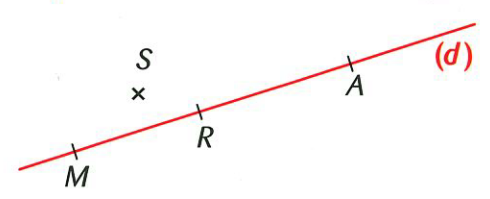
\includegraphics[scale=0.55]{img/droite1}
	\end{center}

	\begin{itemize}
		\item La droite $(d)$ passant par les points $M$ et $R$ se note 
		\item Le point A appartient à la droite $(MR)$, on note :
		\item Le point S n'appartient pas à la droite $(MR)$, on note :
	\end{itemize}
\end{myex}

\begin{mydef}
	Une \kw{demi-droite} est une portion de droite limitée d'un seul côté par un point, son \kw{origine}.
\end{mydef}

\begin{myprop}
	La demi-droite d'origine $A$ et passant par $B$ se note $[AB)$.
\end{myprop}

\begin{myex}
	\begin{center}
		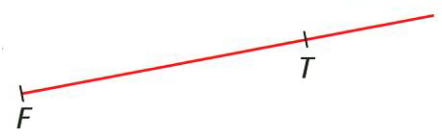
\includegraphics[scale=0.55]{img/demi-droite}
	\end{center}

	La demi droite 
\end{myex}

\begin{mydef}
	Un \kw{segment} est une portion de droite limitée par deux points : ses \kw{extrémités}.
\end{mydef}


\begin{myprop}
	Le segment d'extrémités $A$ et $B$ se note $[AB]$ ou $[BA]$.
\end{myprop}

\begin{myex}
	\begin{center}
		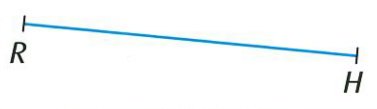
\includegraphics[scale=0.55]{img/segment}
	\end{center}
	
	Le segment 
\end{myex}

\newpage

\section{Longueurs et codages}

\begin{mydefs}
	\iftoggle{eleve}{%
		La mesure \hrulefill
		
		\vspace*{0.2cm}
		\hrulefill 
		
		La longueur \hrulefill
		
	}{%
	La mesure d'un segment (distance entre ses deux extrémités) est sa \kw{longueur}.
	
	La longueur d'un segment $[AB]$, se note $AB$ ou $BA$. 
}
\end{mydefs}


\begin{myex}
	\vspace*{-0.5cm}
	\begin{center}
		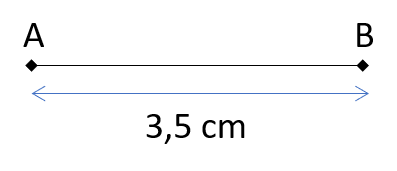
\includegraphics[scale=0.8]{img/lgr}
	\end{center}
	\vspace*{-0.5cm}
	
	\iftoggle{eleve}{%
		La longueur \hrulefill
		\vspace*{0.2cm}
		\hrulefill 
}{%
	La longueur du segment $[AB]$ est de \num{3.5} cm, on note $AB=\num{3.5}$ cm.
}	
	
\end{myex}

\begin{mydef}
	\iftoggle{eleve}{%
		Le \kw{milieu} d'un segment \hrulefill \\
		\vspace*{0.2cm}
		\hrulefill 
	}{%
		Le \kw{milieu} d'un segment est le point qui appartient au segment \kw{et} qui est à égale distance de ses extrémités.
	}
	
\end{mydef}

\begin{myrem}
	\iftoggle{eleve}{%
		Des segments de \hrulefill 
		
		\vspace*{0.2cm}
		\hrulefill 
	}{%
		Des segments de même longueur sont codés de façon identique.
	}
	
\end{myrem}

\begin{myex}
	
	\begin{center}
		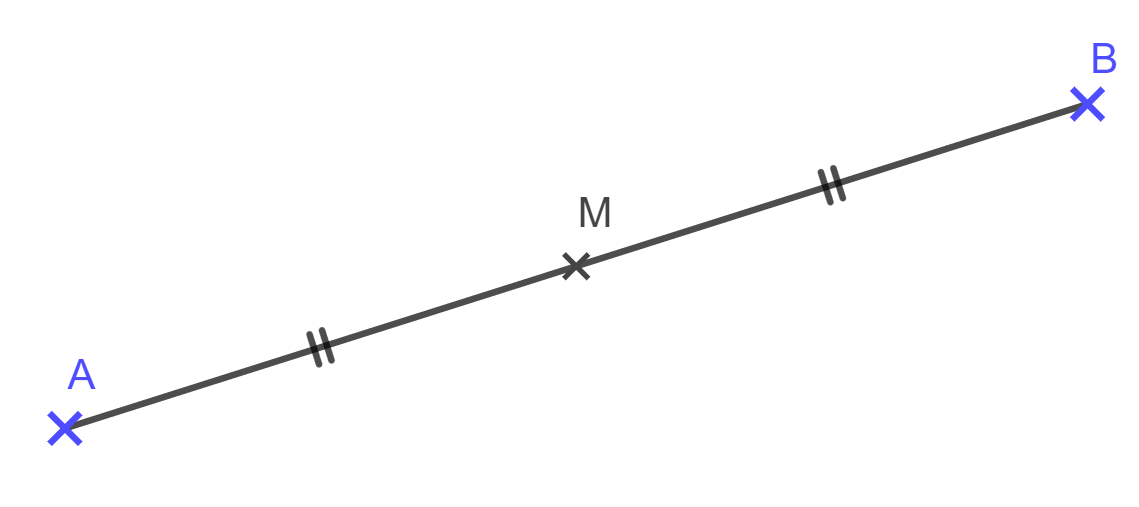
\includegraphics[scale=0.35]{img/milieu}
	\end{center}
	\iftoggle{eleve}{%
		On a : $M \in [AB]$ \hrulefill 
		
		\vspace*{0.2cm}
		\hrulefill 
	}{%
		On a : $M \in [AB]$ et $AM = MB$, donc le point $M$ est le milieu du segment $[AB]$. On a ainsi $AM = AB \div 2$. 
	}

\end{myex}

\section{Sécantes, perpendiculaires et parallèles}

%\begin{mydef}
%	Deux droites sont \kw{sécantes} si elles n'ont qu'un seul point commun : leur \kw{point d'intersection}.
%\end{mydef}
%
%
%\begin{myex}
%	\begin{multicols}{2}
%		Les droites $(d)$ et $(d')$ sont sécantes en $O$ qui est leur point d'intersection.
%		
%		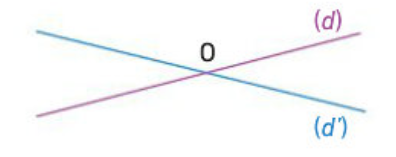
\includegraphics[scale=0.5]{img/sec}
%	\end{multicols}
%	
%\end{myex}
%
%\begin{mydef}
%	Deux droites sont \kw{perpendiculaires} si elles se coupent en formant \kw{quatre angles droits}. Si deux droites $(d_1)$ et $(d_2)$ sont deux droites perpendiculaires, on note $(d_1) \perp (d_2)$.
%\end{mydef}
%
%\begin{myex}
%	\begin{multicols}{2}
%		Les droites $(d)$ et $(d')$ sont perpendiculaires en $H$. $H$ est le pied de la perpendiculaire à $(d')$.
%		
%		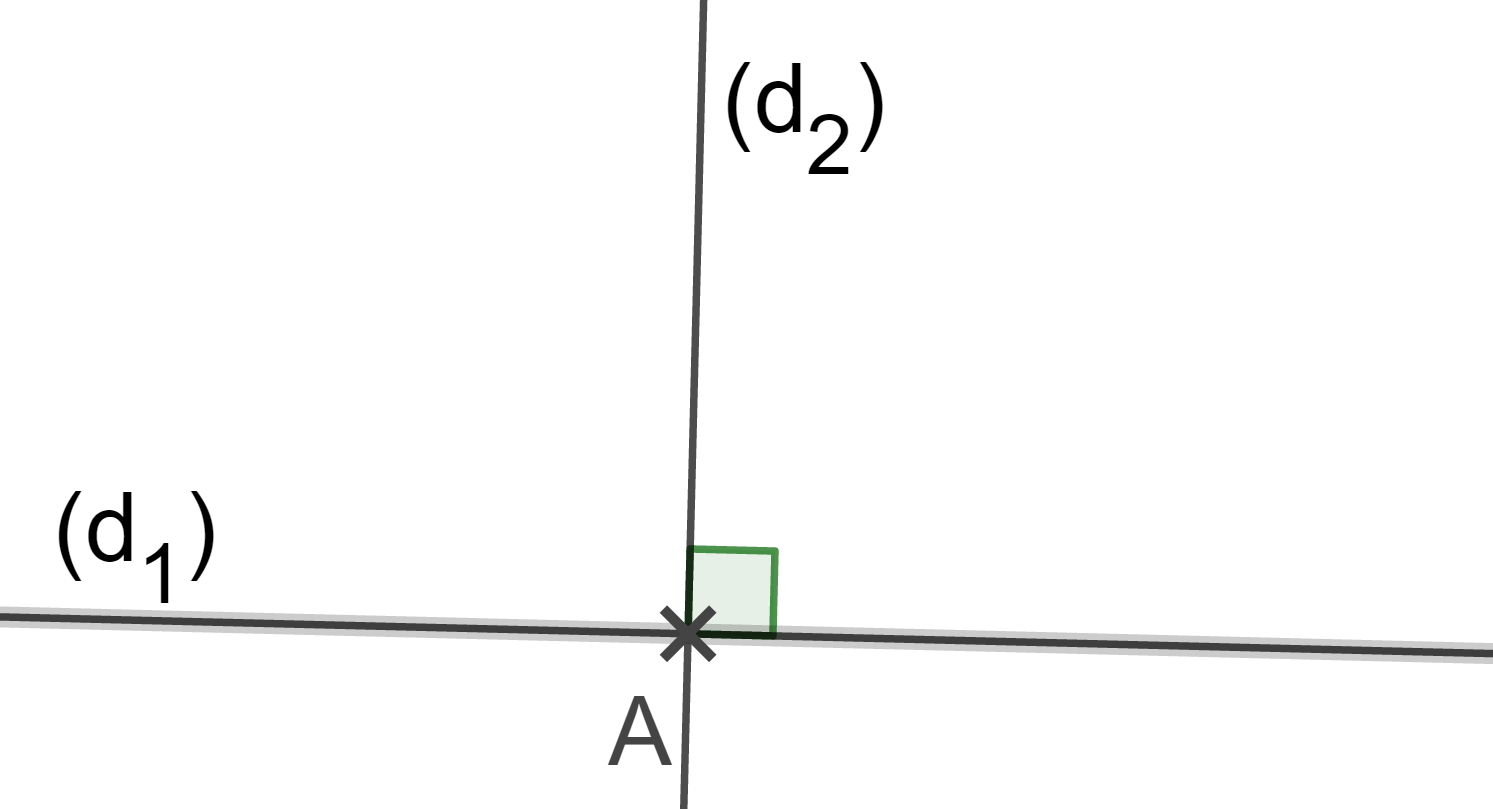
\includegraphics[scale=0.6]{img/perp}
%	\end{multicols}
%	
%\end{myex}
%
%\begin{mydef}
%	Deux droites qui ne sont pas sécantes sont \kw{parallèles}. Si deux droites $(d_3)$ et $(d_4)$ sont parallèles, on note $(d_1) // (d_2)$.
%\end{mydef}
%
%\begin{myex}
%	\begin{multicols}{2}
%		Les droites $(d)$ et $(d')$ sont parallèles. Même en les prolongeant à l'infini elles ne se rencontreront jamais.
%		
%		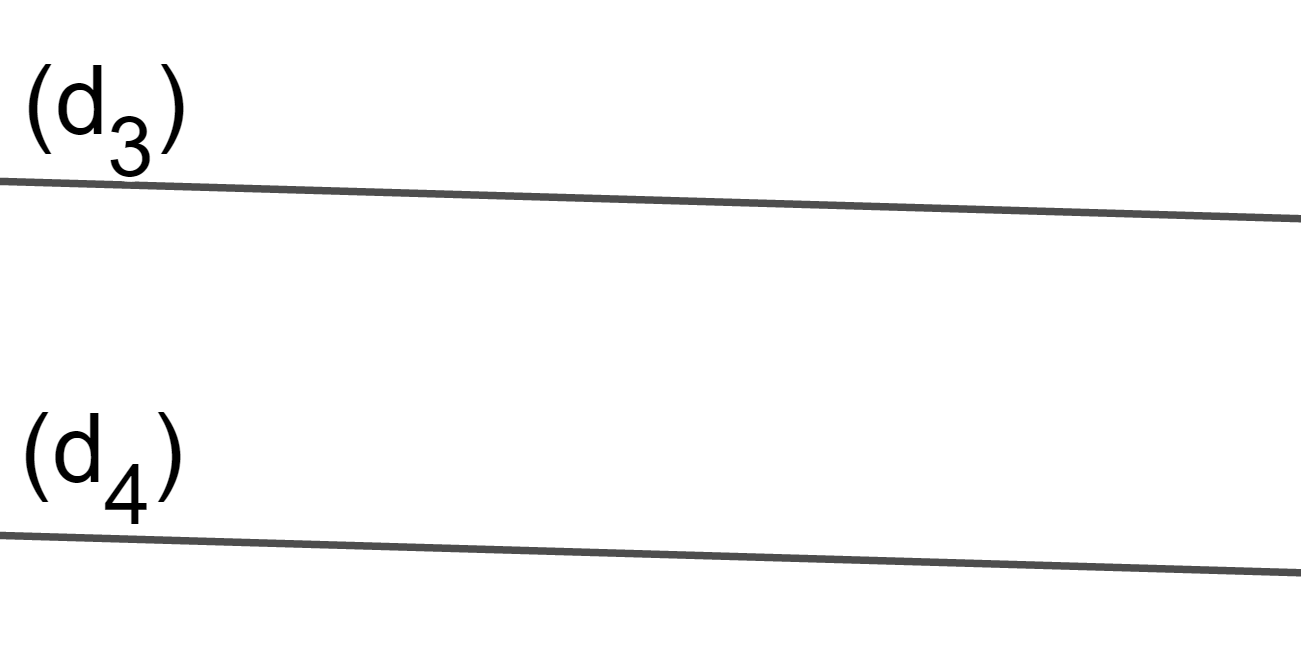
\includegraphics[scale=0.6]{img/para1}
%	\end{multicols}
%	
%\end{myex}
%
%\begin{myprop}
%	\kw{Si} deux droites sont perpendiculaires à une même troisième droite, \kw{alors} ces deux droites sont parallèles.
%\end{myprop}
%
%
%\begin{myex}
%	\begin{multicols}{2}
%		\kw{On sait que} $(d_1)$ et $(d_2)$ sont toutes deux perpendiculaires à $(D)$.\\
%		\kw{Donc} $(d_1)$ et $(d_2)$ sont parallèles.
%		
%		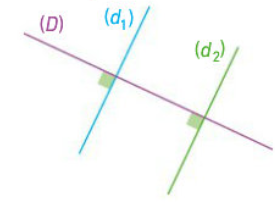
\includegraphics[scale=0.6]{img/para2}
%	\end{multicols}
%	
%\end{myex}



\begin{myprop}
	\kw{Si} deux droites sont parallèles, \kw{alors} toute perpendiculaire à l’une est perpendiculaire à l’autre
\end{myprop}


\begin{myex}
	\begin{multicols}{2}
		\kw{On sait que} $(d_1)$ // $(d_2)$ et $(d_1) \perp (D)$\\
		\kw{Donc} $(d_2) \perp (D)$.
		
		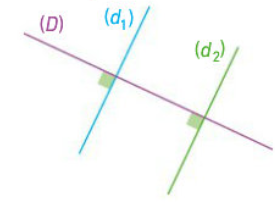
\includegraphics[scale=0.6]{img/para2}
	\end{multicols}
	
\end{myex}

\begin{myprop}
	\kw{Si} deux droites sont parallèles à une même troisième, \kw{alors} ces deux droites sont parallèles entre elles.
\end{myprop}

\begin{myex}
	\begin{multicols}{2}
		\kw{On sait que} $(d_1)$ // $(d)$ et $(d_2) // (d)$\\
		\kw{Donc} $(d_1) \perp (d_2)$.
		
		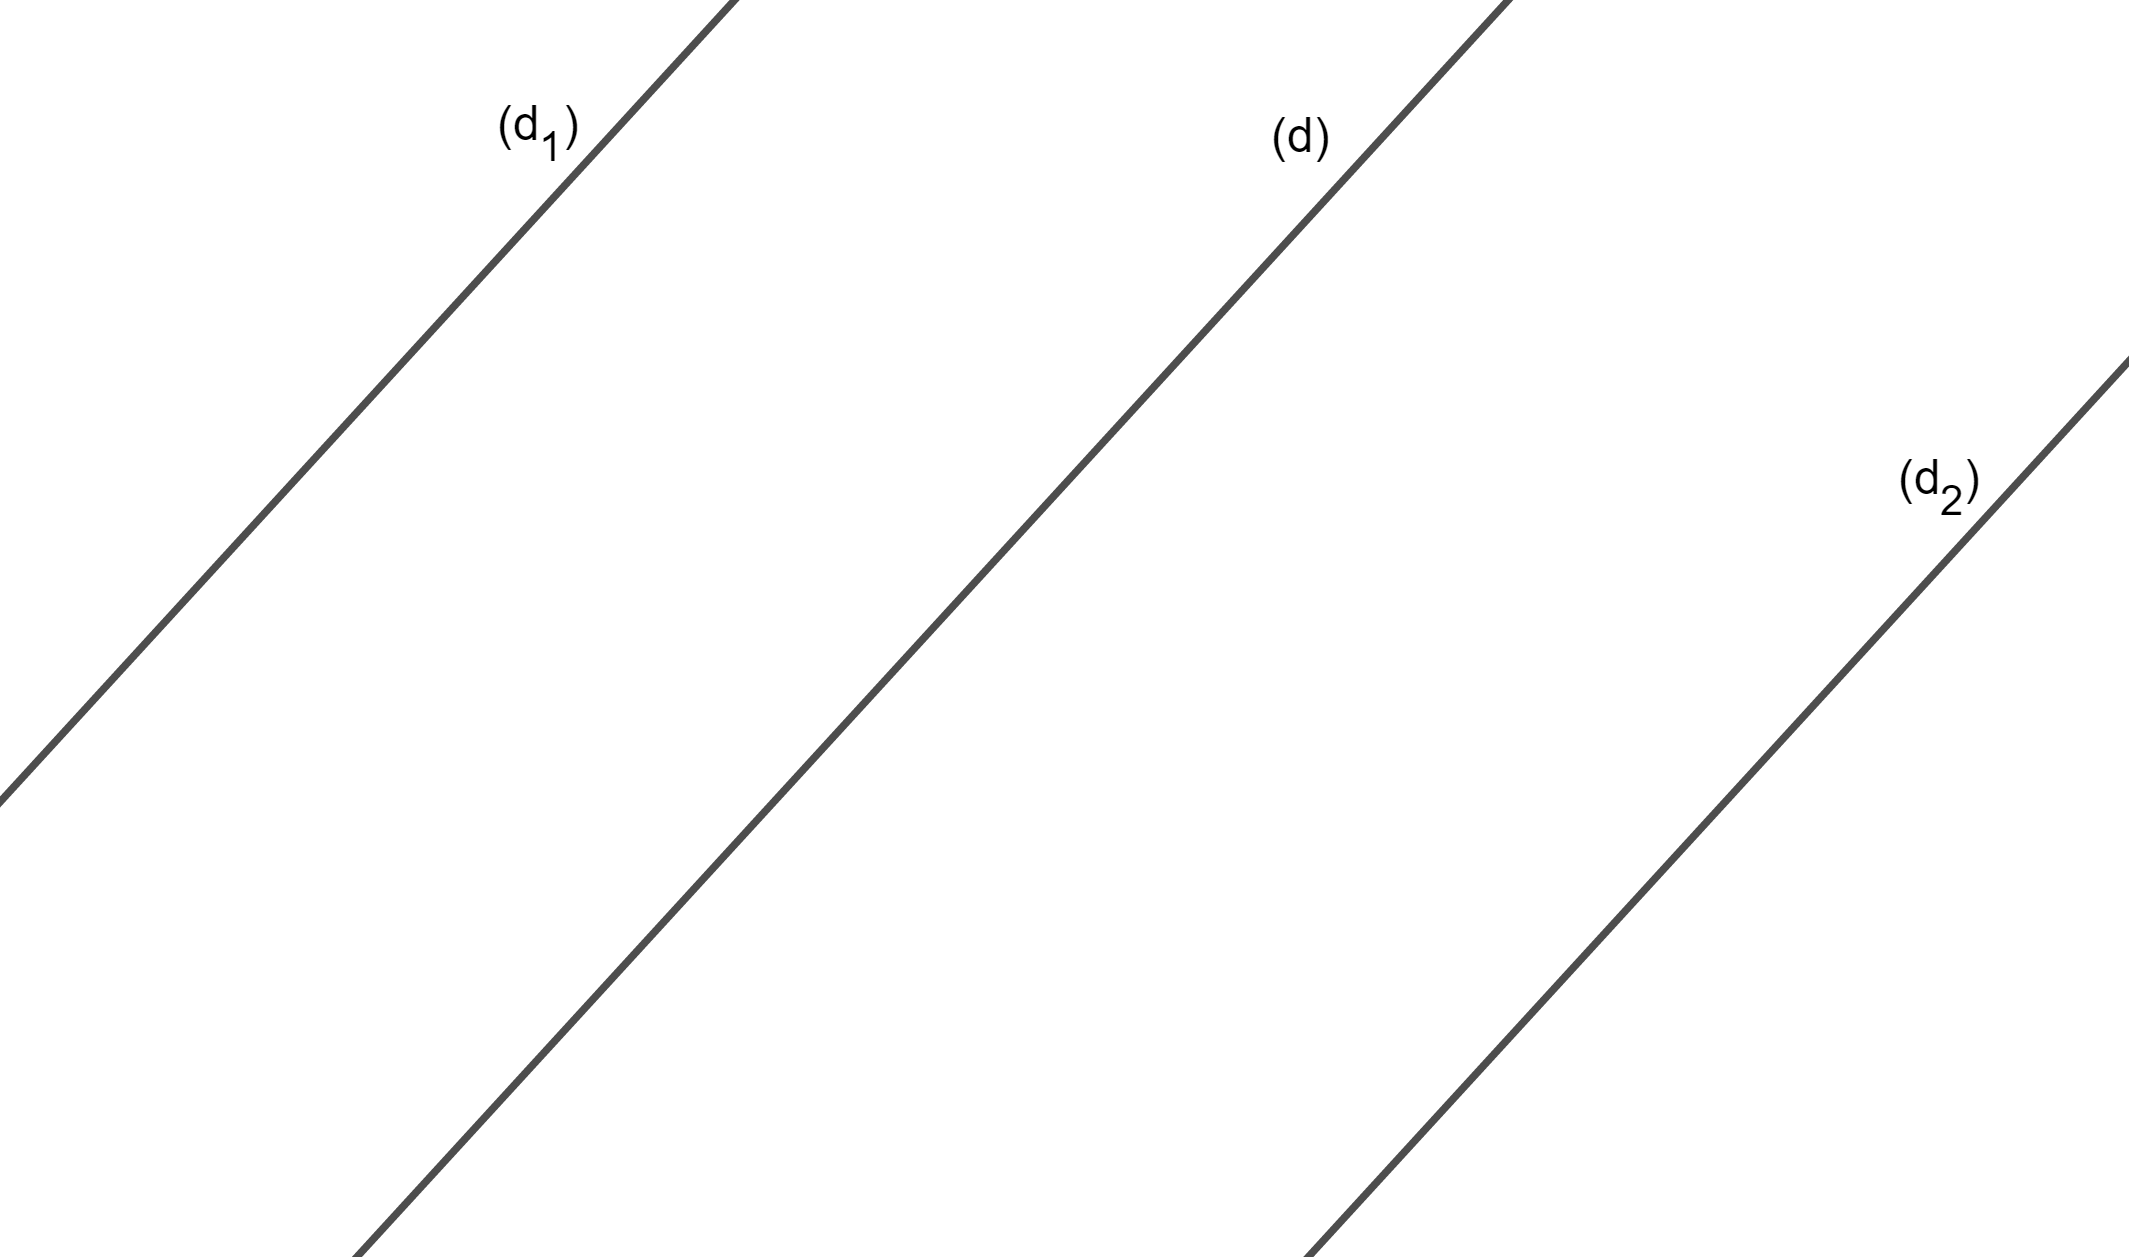
\includegraphics[scale=0.1]{img/para3}
	\end{multicols}
	
\end{myex}

\end{document}